\documentclass[11pt]{article}
\usepackage{UF_FRED_paper_style}
\onehalfspacing

\setlength{\droptitle}{-5em} %% Don't touch

\title{Trabajo II Econometria: Series de Tiempo Multivariadas
}

\author{Augusto Rico\\
    \href{mailto:arico@unal.edu.co}{\texttt{arico@unal.edu.co}}
\and Mauricio Gomez\\% Name author
    \href{mailto:ivmgomezsi@unal.edu.co}{\texttt{ivmgomezsi@unal.edu.co}} %% Email author 2
    }

\date{\today}

\begin{document}

\setstretch{.8} %% Don't touch
\maketitle


% %%%%%%%%%%%%%%%%%%%%%%%%%%%%%%%%%%%%%%%%%%%%%%%%%%%%%%%%%%
% %%%%%%%%%%%%%%%%%%%%%%%%%%%%%%%%%%%%%%%%%%%%%%%%%%%%%%%%%%
% BODY OF THE DOCUMENT
% %%%%%%%%%%%%%%%%%%%%%%%%%%%%%%%%%%%%%%%%%%%%%%%%%%%%%%%%%%
% %%%%%%%%%%%%%%%%%%%%%%%%%%%%%%%%%%%%%%%%%%%%%%%%%%%%%%%%%%

% --------------------
\section{Introduccion}
% --------------------
\begin{flushleft}
    El objetivo principal de este estudio es verificar empíricamente el cumplimiento de ciertas teorías económicas mediante el uso de series de tiempo multiecuacionales. Para ello, utilizaremos dos series de tiempo diarias con 2829 observaciones: la serie del fondo de inversiones \textit{iShares Silver Trust}\footnote{NYSEARCA:SLV}, como indicador del precio de la plata; y la serie del fondo \textit{iShares MSCI Global Silver and Metals Miners} ETF\footnote{BATS:SLVP}, como indicador del valor de empresas mineras dedicadas principalmente a la extracción de plata.

    Estas series nos serán útiles para verificar teorías económicas, como la relacionada con la teoría de la firma y sus beneficios. Según esta teoría, si hay una variación en el precio pero no en las cantidades, debería ocurrir una variación en la misma dirección en los beneficios. Esto afecta el valor intrínseco de la empresa y, por ende, el precio de las acciones de dichas empresas. Si esto se cumple, se espera que los participantes del mercado sean agentes racionales, tal como lo explica la teoría económica mainstream. Por lo tanto, se espera evidenciar una cointegración entre el precio de la plata y el precio de las mineras de plata en el mercado.
    
    Para este estudio, nos respaldamos en un estudio econométrico realizado por \citet{Gilmore_McManus_Sharma_Tezel_2009} sobre el oro. En dicho estudio se encontró la existencia de cointegración entre el precio del oro y las mineras de oro, así como causalidad en esta correlación, con un rápido ajuste frente a las perturbaciones para restablecer la relación de largo plazo entre las variables, hallazgos que contribuyen a la comprensión de las interacciones y dinámicas entre estos activos y respaldan teorías económicas relacionadas. Por lo tanto, en este estudio actual, se verificará si este patrón también se cumple para un metal tan similar en características como la plata.
\end{flushleft}
\section{Cointegracion uniecuacional}
\subsection{analisis visual}
\begin{flushleft}
    \begin{center}
    \begin{figure}[!ht]
      \centering
      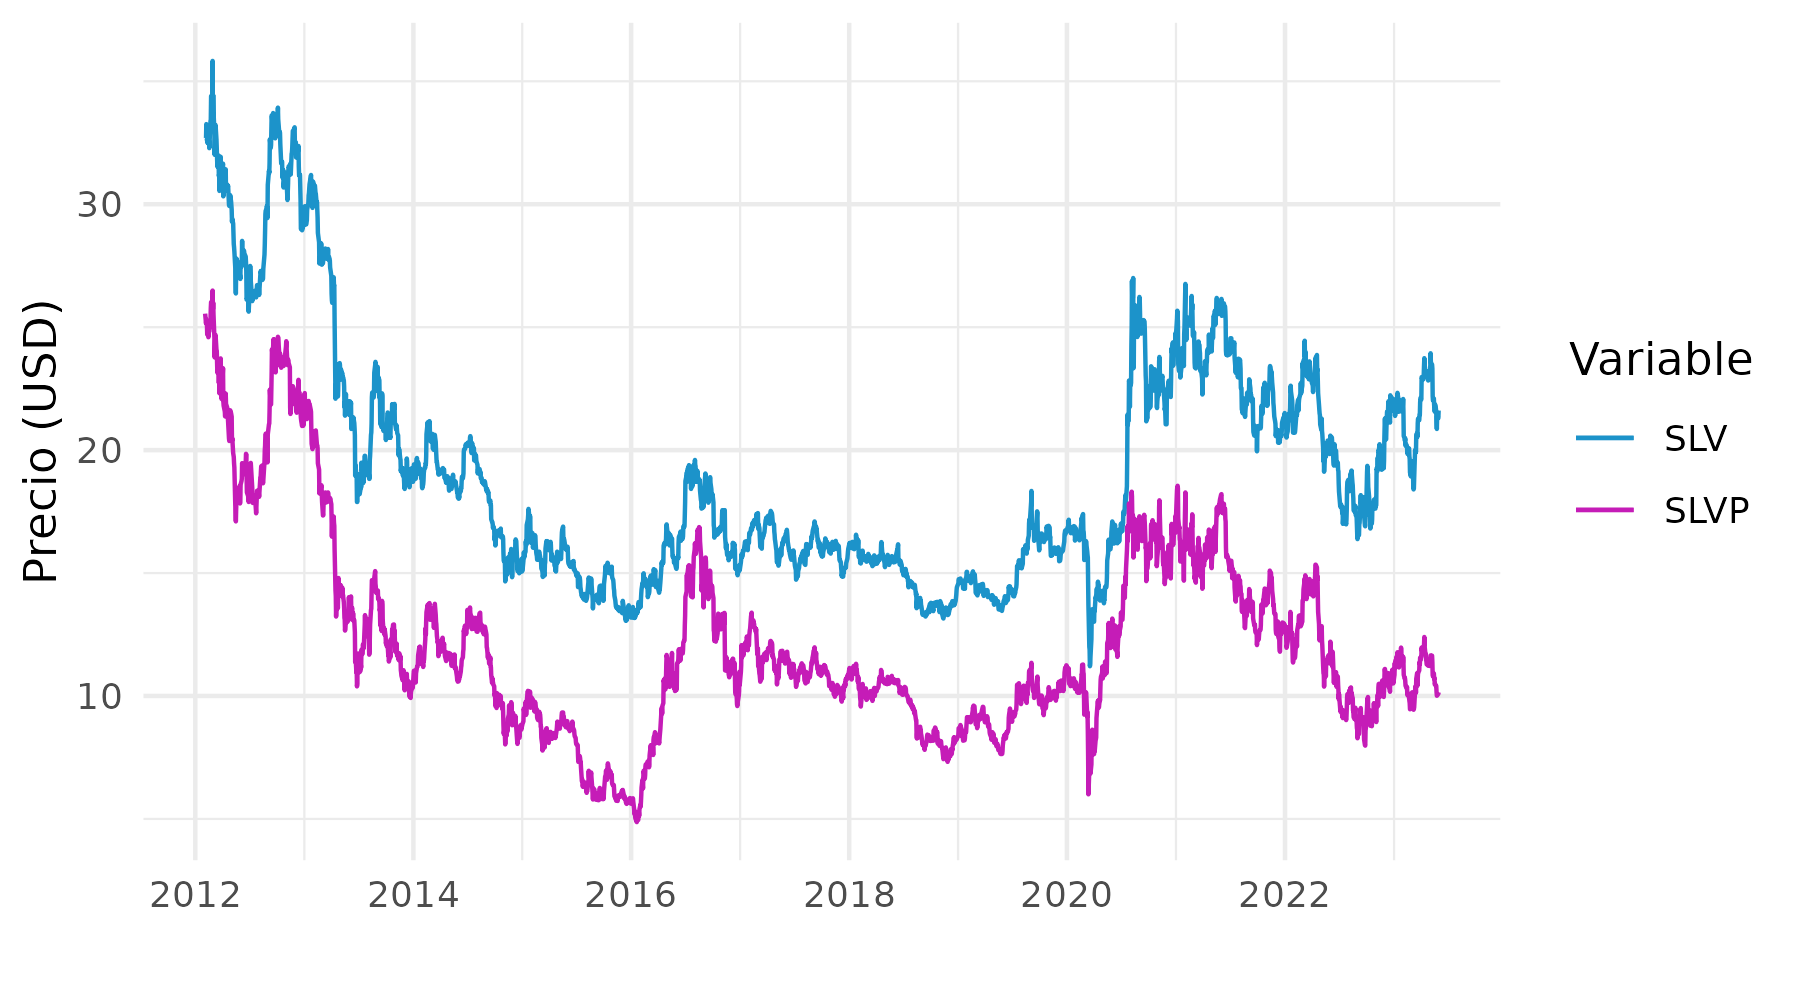
\includegraphics[width=12cm, height=5cm]{Imagenes/ts.png}
      \vspace{0cm}
    \end{figure}
  \end{center}
La primera impresión sugiere una posible cointegración entre las series SLV y SLVP, ya que se observa una notable similitud en su comportamiento en el gráfico. Sin embargo, antes de realizar pruebas de cointegración, es necesario verificar la estacionariedad de las series. A simple vista, también se denota la no estacionariedad de las series, por lo que se utilizarán herramientas econométricas apropiadas para confirmar estas suposiciones.
\end{flushleft}

\subsection{Pruebas de cointegracion}

\begin{flushleft}
    Para realizar las pruebas de Engel-Granger y Johansen correspondientes, es necesario comenzar verificando la estacionariedad de las series. Esto se logra mediante la aplicación de la prueba Dickey-Fuller aumentada a ambas series. Los resultados obtenidos indican que ambas series presentan al menos una raíz unitaria, lo que implica la necesidad de diferenciarlas. Además, se concluye que no se requiere incluir términos de intercepto y tendencia en el modelo, ya que no son estadísticamente significativos.\\~\\
    En particular, al realizar la prueba de raíz unitaria de Dickey-Fuller aumentada, se observa que los estadísticos de prueba para las pruebas con constante y tendencia (trend), solo constante (drift) y sin constante ni tendencia (none) caen en la zona de no rechazo de la hipótesis nula en todos los casos para ambas series, lo que indica la presencia de raíz unitaria.\\~\\
    Después de aplicar la primera diferenciación, se obtienen los estadísticos de prueba de -20.2511 para la serie de SLV y de -20.6704 para la serie de SLVP. Estos valores son inferiores al valor crítico ($1\%$) de -2.58, lo cual lleva al rechazo de la hipótesis nula. Por lo tanto, se concluye que ambas series no tienen raíz unitaria y son estacionarias.\\~\\
    Una vez confirmada la estacionariedad en ambas series tras las transformaciones adecuadas según los resultados de las pruebas ADF, se seleccionan las series transformadas utilizando logaritmos y diferencias, ya que presentan una media y varianza constantes. Con esto, se procede a realizar la prueba de Engel-Granger para verificar la existencia de una relación de cointegración.
\end{flushleft}

\subsubsection{Prueba de Engel-Granger\footnote{veanse todas las tablas de esta prueba en el anexo}}
    \begin{flushleft}
    Para llevar a cabo la prueba de Engle-Granger, se utilizó una regresión de mínimos cuadrados ordinarios dinámicos entre las series. El parámetro de cointegración ($\beta$) obtenido fue de 1.13. Luego se aplicó una prueba de Dickey-Fuller aumentada a los residuos, obteniendo un estadístico de prueba de -2.6643, el cual es menor al valor crítico del $1\%$ -2.58. Por lo tanto, se concluye que el modelo es estacionario y las series están cointegradas.
        \begin{figure}[!ht]
          \centering
          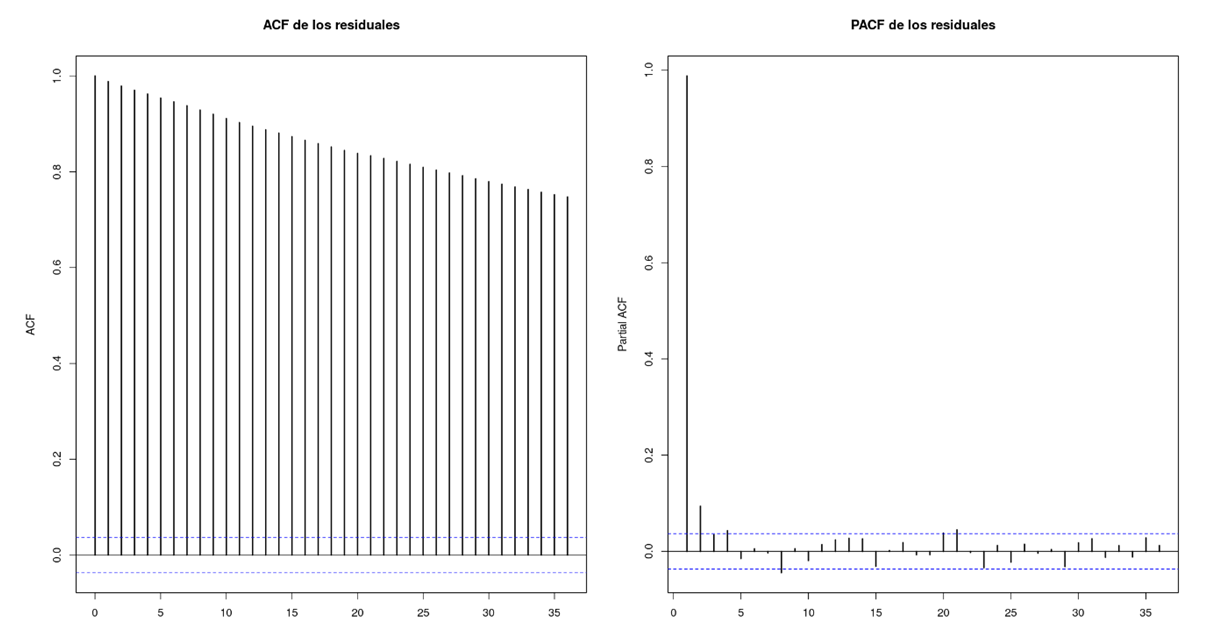
\includegraphics[width=15cm, height=5cm]{Imagenes/ResidualesEG.png}
          \vspace{0cm}
        \end{figure}
    Hecho que también se puede observar al analizar la gráfica de la función de autocorrelación (FAC) de los residuos, es un decaimiento hacia cero, lo cual indica que los residuos son estacionarios. Por lo tanto, se puede concluir que las series están cointegradas.\\~\\
    Finalmente, se realiza la prueba directa utilizando el método de Engle-Granger en R. La conclusión obtenida es que las series están cointegradas, ya que el valor p del tipo 1: no tendencia es menor a 0.05, lo que implica el rechazo de la hipótesis nula en favor de la cointegración.
\end{flushleft}
\subsubsection{Prueba de Johansen}

\begin{minipage}{0.5\textwidth}
\begin{flushleft}
~\\Dado que previamente se ha establecido que las series son $I(1)$, resulta pertinente aplicar el test de Johansen para determinar las relaciones de cointegración existentes.
\end{flushleft}
\end{minipage}
\hfill
\begin{minipage}{0.5\textwidth}
    \centering
    \begin{table}[H]
\centering
\begin{tabular}{|ccccc|}
\hline
\multicolumn{5}{|c|}{\textbf{Test de Johansen: traza }}                                                                                               \\ \hline
\multicolumn{1}{|c|}{}                 & \multicolumn{1}{c|}{test}  & \multicolumn{1}{c|}{10pct} & \multicolumn{1}{c|}{\textbf{5pct}} & 1pct  \\ \hline
\multicolumn{1}{|c|}{r \textless{}= 1} & \multicolumn{1}{c|}{11.16}  & \multicolumn{1}{c|}{6.50}  & \multicolumn{1}{c|}{8.18}          & 11.65 \\ \hline
\multicolumn{1}{|c|}{r = 0}            & \multicolumn{1}{c|}{25.13} & \multicolumn{1}{c|}{15.66} & \multicolumn{1}{c|}{17.95}         & 23.52 \\ \hline
\end{tabular}
\end{table}
\end{minipage}
 Al aplicar la prueba mediante criterios de valores propios y de traza, se concluye que existe más de una relación de cointegración. Esto confirma la conclusión obtenida previamente mediante la prueba de Engel-Granger.
\subsection{modelo VECM}
\begin{flushleft}
    Debido a los resultados anteriores y al estimar las series en niveles y utilizar criterios de información sin términos determinísticos para seleccionar el modelo VAR adecuado, hemos procedido a realizar la estimación del modelo VECM(1) en diferencias.\\~\\

    Luego, validamos este modelo a partir del modelo VAR. Para llevar a cabo esta validación, examinamos el comportamiento del modelo y realizamos pruebas para verificar la presencia o ausencia de autocorrelación, homocedasticidad y normalidad mediante el Test Jarque-Bera multivariado.\\~\\
    
    Observamos que el modelo presenta problemas de correlación serial, homocedasticidad y normalidad. Sin embargo, al observar el FAC y FACP de los residuos, evidenciamos que el problema de correlación serial no es realmente grave.
\end{flushleft}
    
\subsection{MCOD}
\begin{flushleft}
    Se utilizó la primera ecuación con la tasa de cambio como variable dependiente en el modelo de corrección de errores dinámicos. El análisis basado en el criterio AIC determinó que el número óptimo de rezagos es 6. El coeficiente de regresión estimado por MCOD es $\beta=0.76$, lo que sugiere una relación positiva a largo plazo.
    En cuanto a los supuestos de validación, el modelo cumple con la condición de no autocorrelación, pero se rechaza la hipótesis nula para los supuestos de no heterocedasticidad y normalidad, lo que indica que el modelo no satisface estos últimos.
\end{flushleft}

\section{Estimación del Modelo VAR}
\begin{flushleft}
    Se estimó un modelo VAR en diferencias basado en pruebas previas y en el amplio respaldo empírico que respalda el uso de este tipo de modelos para series financieras, las cuales suelen presentar estacionariedad \citep{Tsay_2005}.\\~\\
    Como paso inicial, se procedió a seleccionar la cantidad adecuada de rezagos a incluir mediante la estimación de múltiples modelos VAR.\footnote{vease tabla en el anexo} Se excluyeron los términos determinísticos debido a que las pruebas ADF no mostraron evidencia significativa de deriva o tendencia después de la diferenciación. Se utilizó un valor máximo de p de 6 y se empleó la información de los criterios y la búsqueda de parsimonia para calibrar un modelo con solo 1 rezago.\\~\\
    En la validación de supuestos, se encontró que la serie no presenta una autocorrelación serial intensa, pero sí presenta problemas de normalidad y heterocedasticidad, hecho que es coherente con la teoría de las series financieras \citep{Calderon}. Este hallazgo, junto con la ortogonalización de los impulsos, permite obtener análisis causales de las \textit{impulso-respuesta}\\~\\

    \begin{center}
    \begin{figure}[!ht]
      \centering
      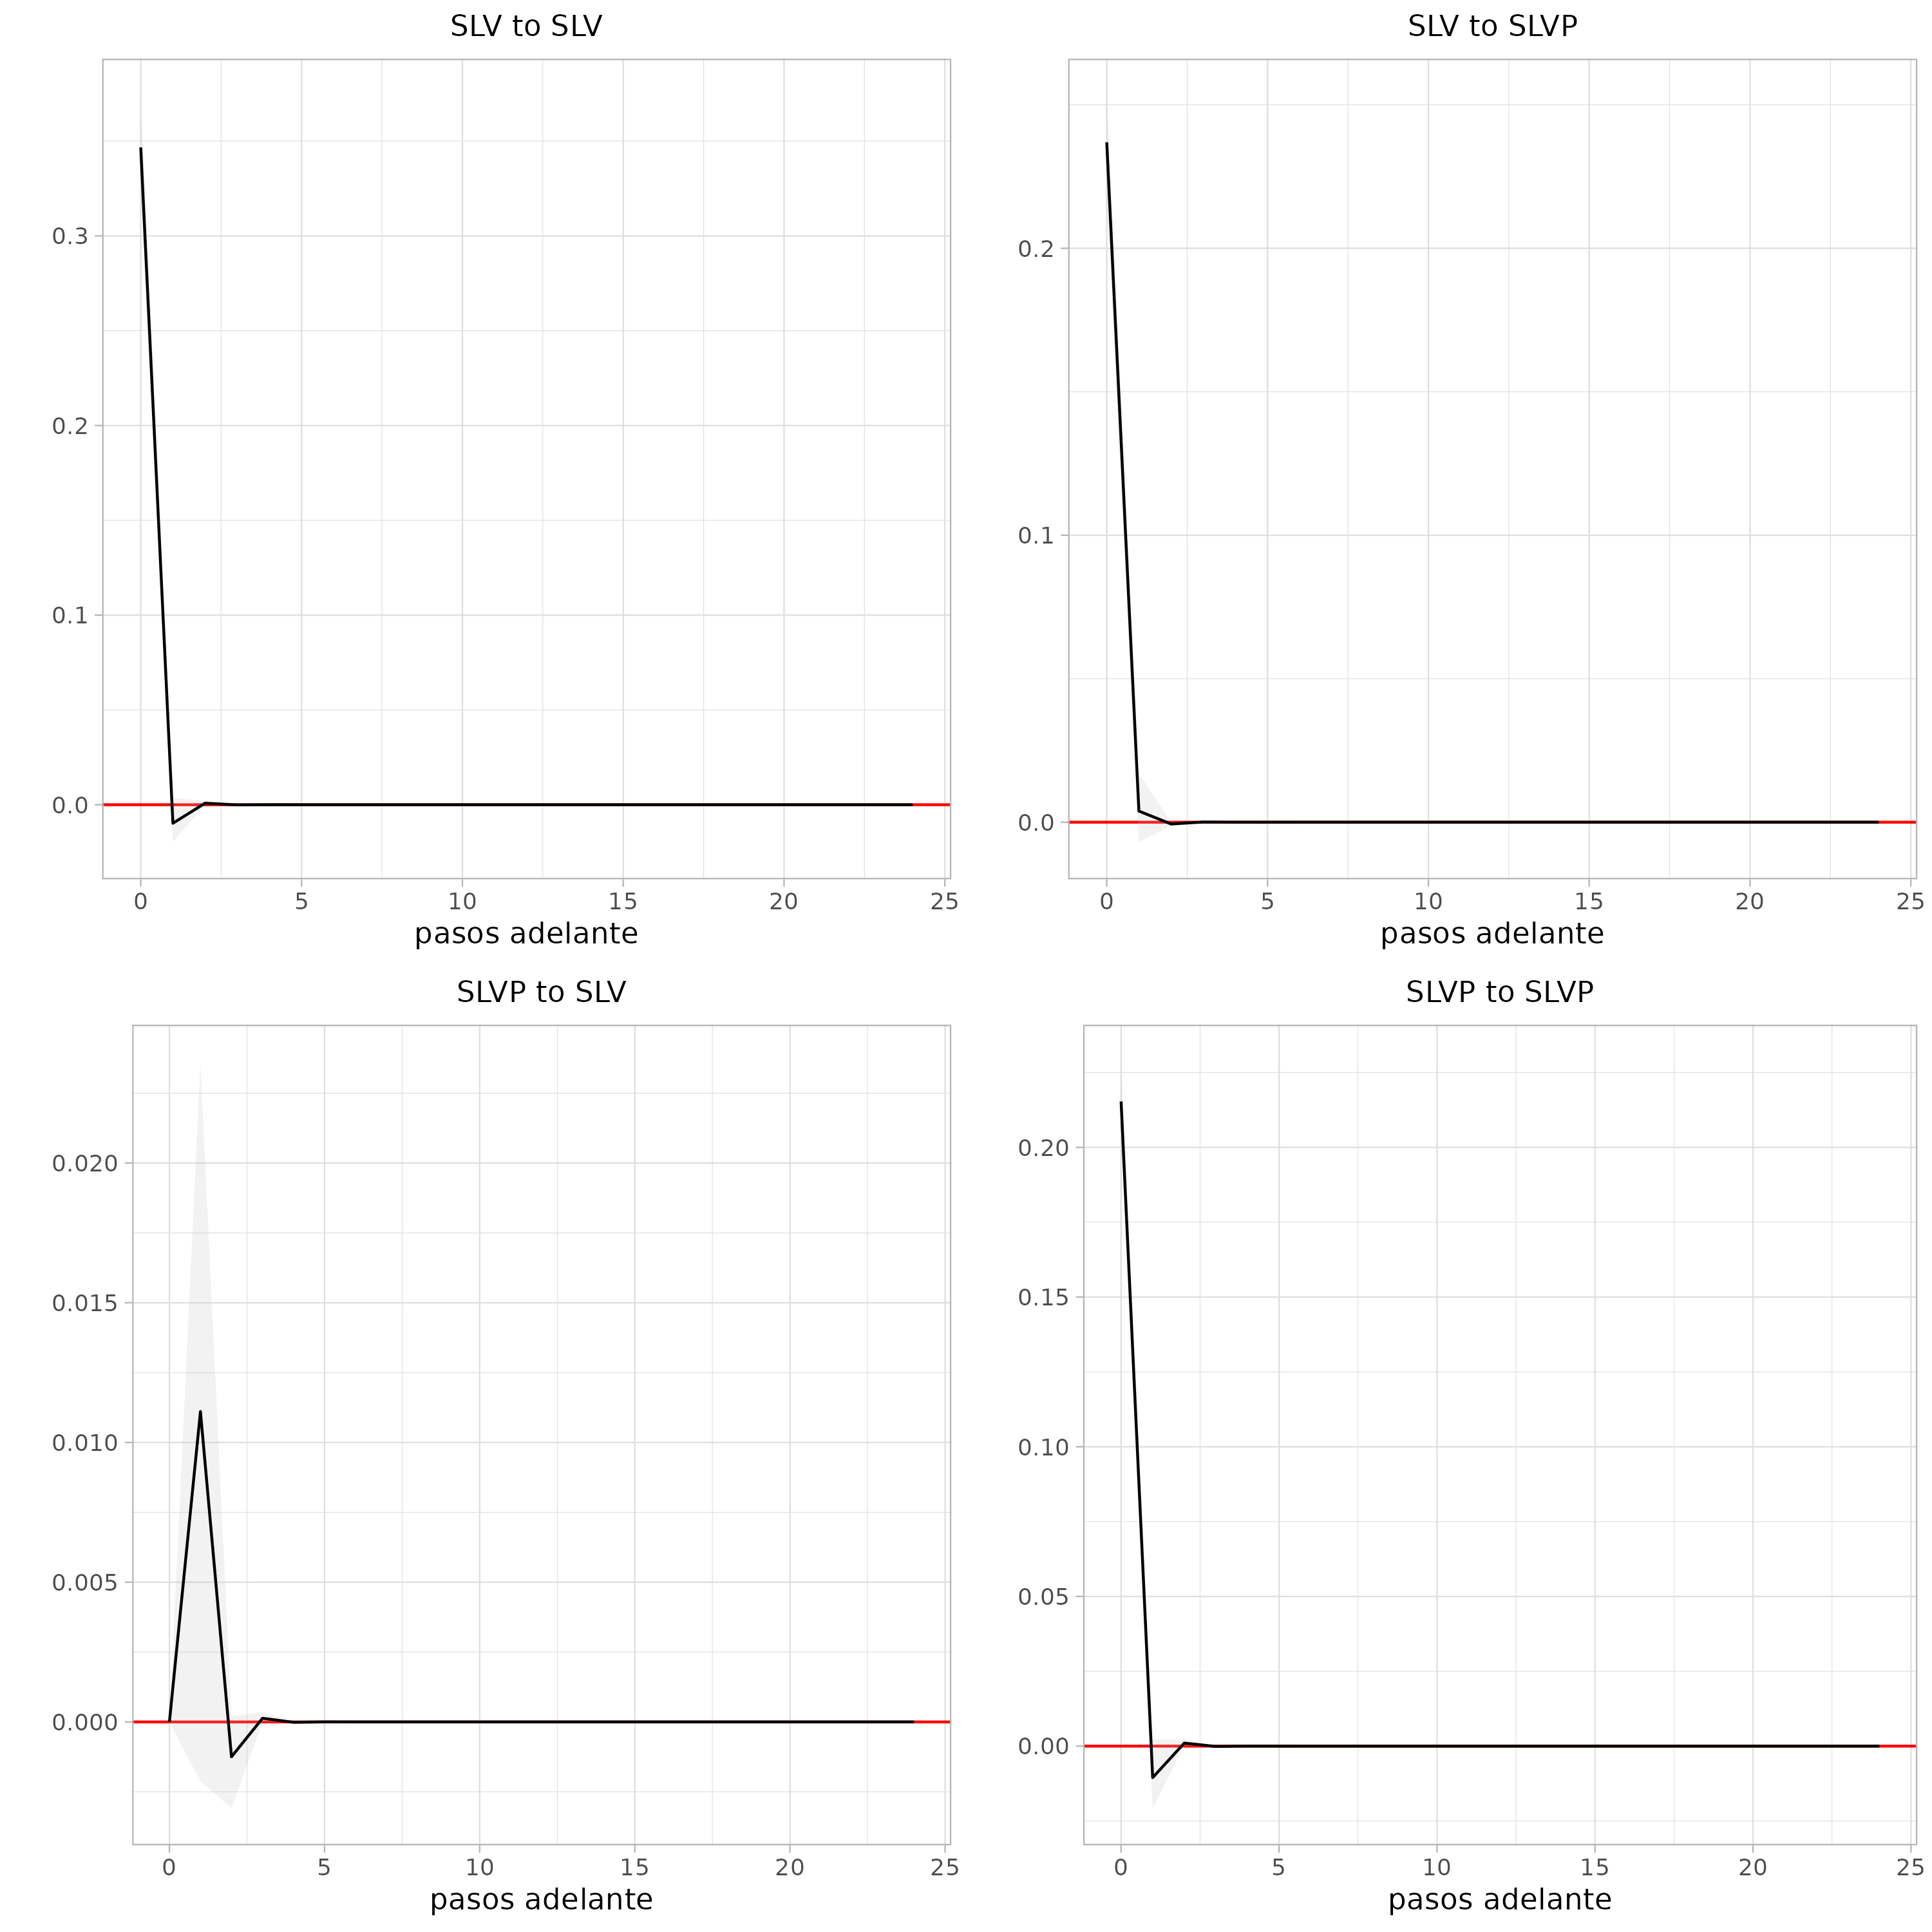
\includegraphics[width=15cm, height=8cm]{Imagenes/impulso_respuesta.png}
      \vspace{0cm}
    \end{figure}
  \end{center}

  de esta grafica se concluye que, todo lo expuesto en la introduccion se cumple, por lo que, como era de esperarse, la plata tiene un comportamiento cointegrado como el del oro tal como expuso \citep{Gilmore_McManus_Sharma_Tezel_2009}, por lo que podemos concluir entonces que:
    \begin{itemize}
        \item Un choque en el precio de la plata provoca un impacto acelerado en los primeros períodos, pero regresa rápidamente a su media de equilibrio, lo que resulta en una baja significancia del choque a largo plazo.
        \item Si el precio de la plata experimenta una caída que afecta el valor de las acciones mineras de plata, se observa un impacto inicial significativo, lo que sugiere una relación causal coherente con la teoría. No obstante, esta situación tiende a ajustarse rápidamente y restablecerse a largo plazo, como se evidencia por la falta de significancia en el largo plazo.
        \item Si, por el contrario, deseamos observar el efecto de un impulso en el precio de las empresas mineras de plata, notaremos que este efecto es prácticamente marginal, hasta el punto de considerarse estadísticamente insignificante. Esto concuerda con la teoría y muestra que el impacto es unidireccional. Por lo tanto, se puede afirmar que la variación en el precio de la plata causa, en términos de la relación de Wiener-Granger, cambios en el precio de las acciones mineras, pero no se puede afirmar lo contrario.
        \item Finalmente, la reacción de un choque en el precio de las empresas mineras sobre ellas mismas alcanza un gran impacto inmediato que pocos periodos después puede generar un muy pequeño impacto negativo, diluyendo la significancia del mismo rápidamente y recuperando la senda de equilibrio con rapidez en pocos periodos.
    \end{itemize}
\end{flushleft}

\section{Conclusiones}

\begin{flushleft}
    \begin{enumerate}
        \item Es posible utilizar modelos de series de tiempo multivariadas para determinar la cointegración entre diferentes series de tiempo.
        \item Al emplear procesos de inferencia en series de tiempo, se ha logrado demostrar la existencia de una relación causal entre el precio de la plata y el precio de las acciones de las empresas mineras de plata.
        \item Utilizando los procesos de inferencia en series de tiempo, se ha comprobado que la relación causal opuesta, en la que el precio de las acciones de las empresas mineras de plata afecta el precio de la plata, no es válida.
        \item En consecuencia, se puede concluir que la relación de impacto es unidireccional y, por lo tanto, se trata de una relación Wiener-Granger, similar a la que existe con el oro.
        \item Esta relación de causalidad también respalda la validez de la función de beneficios de la firma neoclásica en un equilibrio parcial.
        \item Dado que los mercados financieros son mercados con costos de información de los precios casi nulos, se observa cómo estos se ajustan rápidamente ante cambios repentinos, lo que restablece nuevamente las relaciones de largo plazo.
    \end{enumerate}
\end{flushleft}

\newpage

% %%%%%%%%%%%%%%%%%%%%%%%%%%%%%%%%%%%%%%%%%%%%%%%%%%%%%%%%%%
% %%%%%%%%%%%%%%%%%%%%%%%%%%%%%%%%%%%%%%%%%%%%%%%%%%%%%%%%%%
% REFERENCES SECTION
% %%%%%%%%%%%%%%%%%%%%%%%%%%%%%%%%%%%%%%%%%%%%%%%%%%%%%%%%%%
% %%%%%%%%%%%%%%%%%%%%%%%%%%%%%%%%%%%%%%%%%%%%%%%%%%%%%%%%%%
\medskip

\bibliography{references.bib} 

\newpage

\section{Anexos}

    \begin{figure}[!ht]
      \centering
      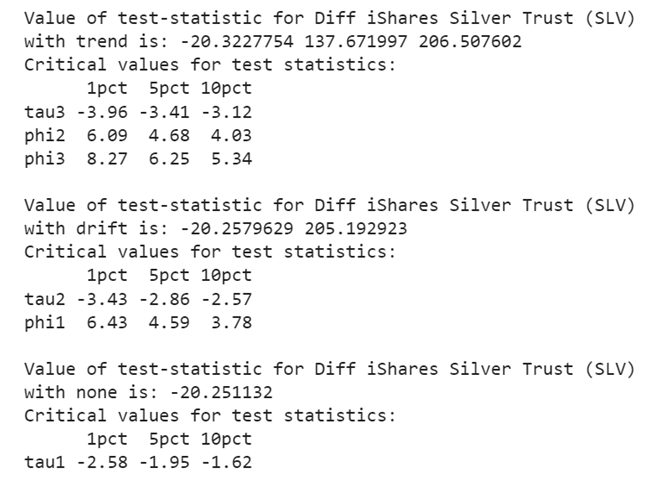
\includegraphics[width=12cm, height=9cm]{Imagenes/1er diff SLV.png}
      \label{fig:Anexo}
      \caption{Primera diferenciación SLV}
      \vspace{0cm}
    \end{figure}

    \begin{figure}[!ht]
      \centering
      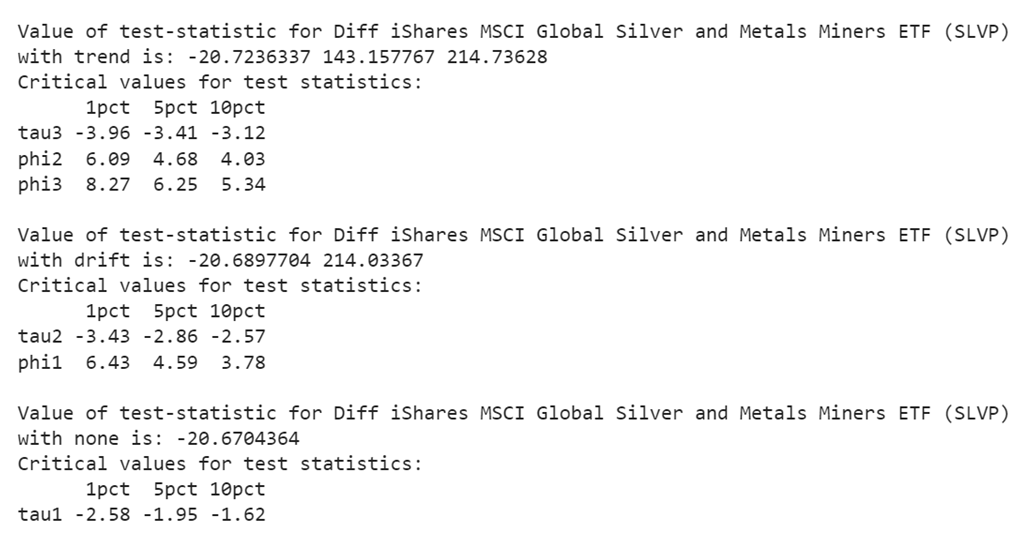
\includegraphics[width=16cm, height=9cm]{Imagenes/1er diff SLVP.png}
      \label{fig:Anexo}
      \caption{Primera diferenciación SLVP}
      \vspace{0cm}
    \end{figure}

    \begin{figure}[!ht]
      \centering
      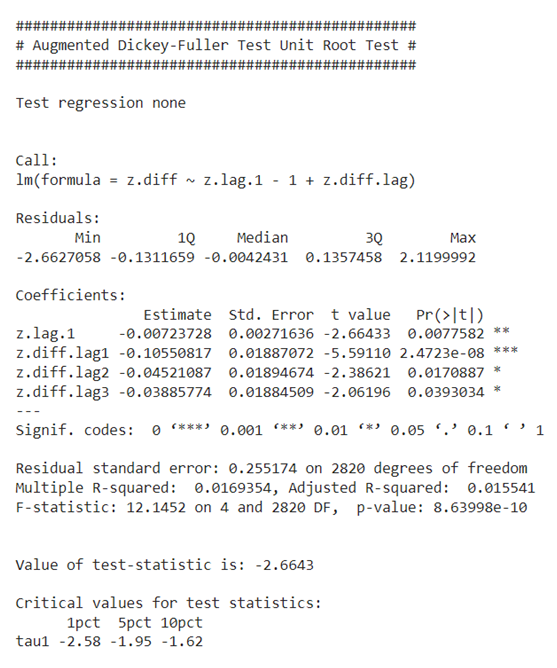
\includegraphics[width=13cm, height=16cm]{Imagenes/DF residualesEG.png}
      \label{fig:Anexo}
       \caption{Prueba Dickey-Fuller sobre los residuales}
      \vspace{0cm}
    \end{figure}
    \begin{figure}[!ht]
      \centering
      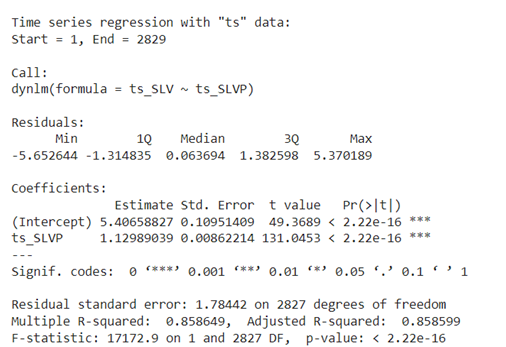
\includegraphics[width=9cm, height=7cm]{Imagenes/MCO.png}
      \label{fig:Anexo}
      \vspace{0cm}
    \end{figure}
    \begin{figure}[!ht]
      \centering
      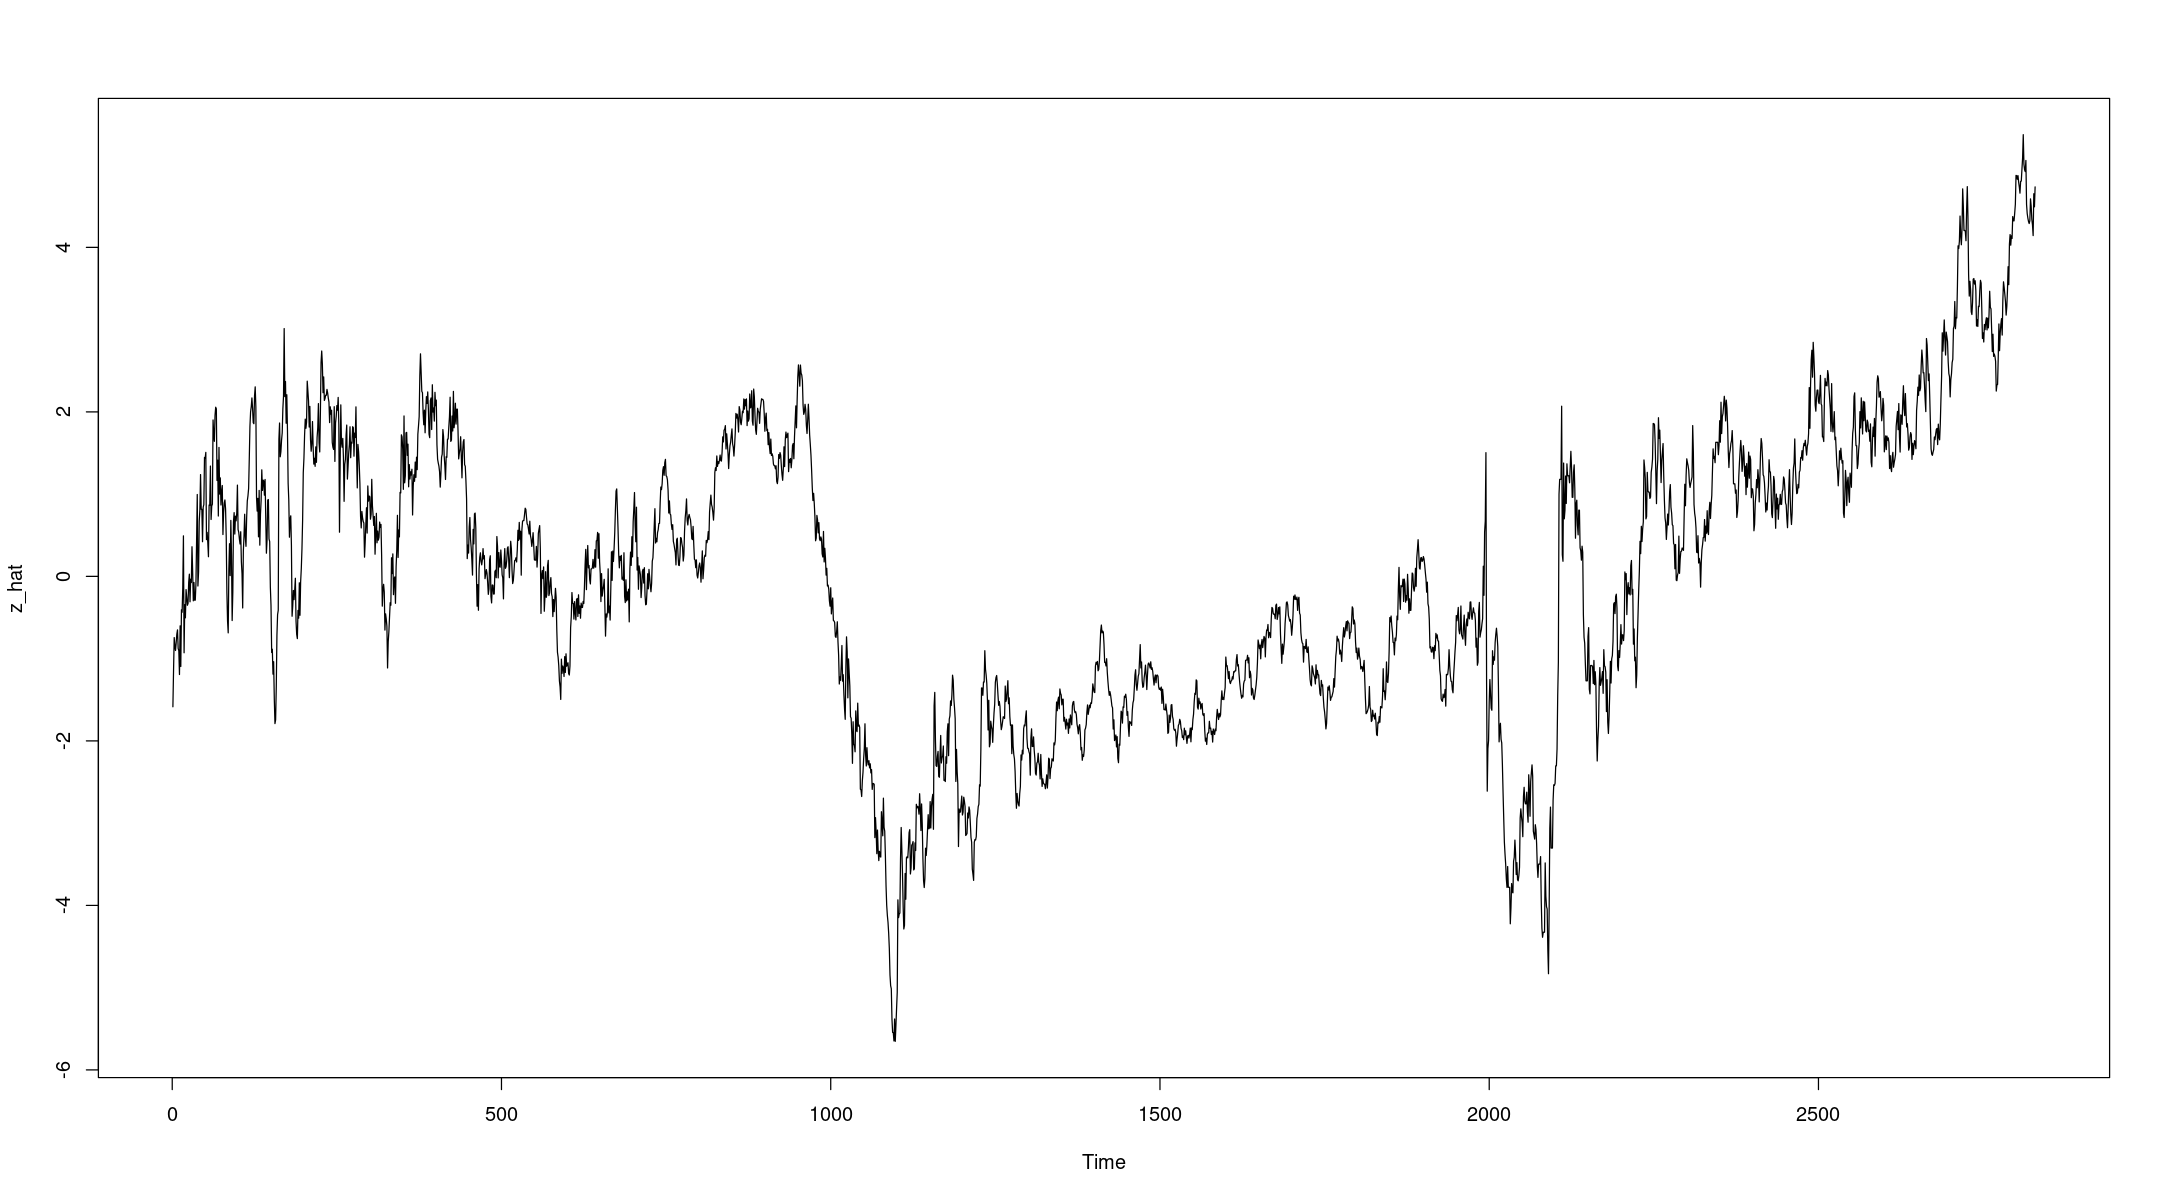
\includegraphics[width=10cm, height=4cm]{Imagenes/z_hat.png}
      \label{fig:Anexo}
      \vspace{0cm}
    \end{figure}
    

\end{document}